% BU ECE template for MS thesis and PhD dissertation.
%
%==========================================================================%
% MAIN PREAMBLE 
%==========================================================================%
\documentclass[12pt,letterpaper]{report}          % Single-sided printing for the library
%\documentclass[12pt,twoside]{report} % Double-sided printing
\usepackage[intlimits]{amsmath}
\usepackage{amsfonts,amssymb}
\DeclareSymbolFontAlphabet{\mathbb}{AMSb}
%\usepackage{natbib}
\usepackage{apalike}
\usepackage{float}
\usepackage[bf]{caption}       
\setcaptionmargin{0.5in}
\usepackage{fancyhdr}
%\usepackage{fancyheadings}
\usepackage{fancybox}
\usepackage{ifthen}
\usepackage{bu_ece_thesis}
\usepackage{url}
\usepackage{lscape,afterpage}
\usepackage{xspace}
\usepackage{epstopdf} 
\usepackage{subfig}
%==========================================================================%
%%% graphicx and pdf creation
\usepackage{graphicx}
\usepackage{appendix}
%\usepackage{psfrag}
%\DeclareGraphicsExtensions{.eps}   % extension for included graphics
%\usepackage{thumbpdf}              % thumbnails for ps2pdf
%\usepackage[ps2pdf,                % hyper-references for ps2pdf
%bookmarks=true,%                   % generate bookmarks ...
%bookmarksnumbered=true,%           % ... with numbers
%hypertexnames=false,%              % needed for correct links to figures !!!
%breaklinks=true,%                  % breaks lines, but links are very small
%linkbordercolor={0 0 1},%          % blue frames around links
%pdfborder={0 0 112.0}]{hyperref}%  % border-width of frames 
%                                   % will be multiplied with 0.009 by ps2pdf
%\hypersetup{
%  pdfauthor   = {Joe Graduate <joe.graduate@bu.edu>},
%  pdftitle    = {dissertation.pdf},
%  pdfsubject  = {doctoral dissertations},
%  pdfkeywords = {mathematics, science, technology},
%  pdfcreator  = {LaTeX with hyperref package},
%  pdfproducer = {dvips + ps2pdf}
%}
%==========================================================================%
% customized commands can be placed here
%\newcommand{\figref}[1]{Figure~\ref{#1}}
%\newcommand{\chapref}[1]{Chapter~\ref{#1}}
%\newcommand{\latex}{\LaTeX\xspace}
%==========================================================================%

%==========================================================================%
% BEGIN
%==========================================================================%
\begin{document}

% The preliminary pages
% This file contains all the necessary setup and commands to create
% the preliminary pages according to the buthesis.sty option.

\title{A BU Thesis Latex Template}

\author{Joe Candidate}

% Type of document prepared for this degree:
%   1 = Master of Science thesis,
%   2 = Doctor of Philisophy dissertation.
%   3 = Master of Science thesis and Doctor of Philisophy dissertation.
\degree=2

\prevdegrees{B.S., Some University, 2010\\
	M.S., Another University, 2012}

\department{Department of Electrical and Computer Engineering}

% Degree year is the year the diploma is expected, and defense year is
% the year the dissertation is written up and defended. Often, these
% will be the same, except for January graduation, when your defense
% will be in the fall of year X, and your graduation will be in
% January of year X+1
\defenseyear{2015}
\degreeyear{2015}

% For each reader, specify appropriate label {First, Second, Third},
% then name, and title. IMPORTANT: The title should be:
%   "Professor of Electrical and Computer Engineering",
% or similar, but it MUST NOT be:
%   Professor, Department of Electrical and Computer Engineering"
% or you will be asked to reprint and get new signatures.
% Warning: If you have more than five readers you are out of luck,
% because it will overflow to a new page. You may try to put part of
% the title in with the name.
\reader{First}{First M. Last, PhD}{Professor of Electrical and Computer Engineering}
\reader{Second}{First M. Last}{Associate Professor of \ldots}
\reader{Third}{First M. Last}{Assistant Professor of \ldots}

% The Major Professor is the same as the first reader, but must be
% specified again for the abstract page. Up to 4 Major Professors
% (advisors) can be defined. 
\numadvisors=2
\majorprof{First M. Last, PhD}{{Professor of Electrical and Computer Engineering\\Secondary appointment}}
\majorprofb{First M. Last, PhD}{{Professor of Computer Science}}
%\majorprofc{First M. Last, PhD}{{Professor of Astronomy}}
%\majorprofd{First M. Last, PhD}{{Professor of Biomedical Engineering}}

%%%%%%%%%%%%%%%%%%%%%%%%%%%%%%%%%%%%%%%%%%%%%%%%%%%%%%%%%%%%%%%%  

%                       PRELIMINARY PAGES
% According to the BU guide the preliminary pages consist of:
% title, copyright (optional), approval,  acknowledgments (opt.),
% abstract, preface (opt.), Table of contents, List of tables (if
% any), List of illustrations (if any). The \tableofcontents,
% \listoffigures, and \listoftables commands can be used in the
% appropriate places. For other things like preface, do it manually
% with something like \newpage\section*{Preface}.

% This is an additional page to print a boxed-in title, author name and
% degree statement so that they are visible through the opening in BU
% covers used for reports. This makes a nicely bound copy. Uncomment only
% if you are printing a hardcopy for such covers. Leave commented out
% when producing PDF for library submission.
%\buecethesistitleboxpage

% Make the titlepage based on the above information.  If you need
% something special and can't use the standard form, you can specify
% the exact text of the titlepage yourself.  Put it in a titlepage
% environment and leave blank lines where you want vertical space.
% The spaces will be adjusted to fill the entire page.
\maketitle
\cleardoublepage

% The copyright page is blank except for the notice at the bottom. You
% must provide your name in capitals.
\copyrightpage
\cleardoublepage

% Now include the approval page based on the readers information
\approvalpage
\cleardoublepage

% Here goes your favorite quote. This page is optional.
\newpage
%\thispagestyle{empty}
\phantom{.}
\vspace{4in}

\begin{singlespace}
\begin{quote}
  \textit{Facilis descensus Averni;}\\
  \textit{Noctes atque dies patet atri janua Ditis;}\\*
  \textit{Sed revocare gradum, superasque evadere ad auras,}\\
  \textit{Hoc opus, hic labor est.}\hfill{Virgil (from Don's thesis!)}
\end{quote}
\end{singlespace}

% \vspace{0.7in}
%
% \noindent
% [The descent to Avernus is easy; the gate of Pluto stands open night
% and day; but to retrace one's steps and return to the upper air, that
% is the toil, that the difficulty.]

\cleardoublepage

% The acknowledgment page should go here. Use something like
% \newpage\section*{Acknowledgments} followed by your text.
\newpage
\section*{\centerline{Acknowledgments}}
Here go all your acknowledgments. You know, your advisor, funding agency, lab
mates, etc., and of course your family.

As for me, I would like to thank Jonathan Polimeni for cleaning up old LaTeX
style files and templates so that Engineering students would not have to suffer
typesetting dissertations in MS Word. Also, I would like to thank IDS/ISS
group (ECE) and CV/CNS lab graduates for their contributions and tweaks to this
scheme over the years (after many frustrations when preparing their final
document for BU library). In particular, I would like to thank Limor Martin who
has helped with the transition to PDF-only dissertation format (no more printing
hardcopies -- hooray !!!)

The stylistic and aesthetic conventions implemented in this LaTeX
thesis/dissertation format would not have been possible without the help from
Brendan McDermot of Mugar library and Martha Wellman of CAS.

Finally, credit is due to Stephen Gildea for the MIT style file off which this
current version is based, and Paolo Gaudiano for porting the MIT style to one
compatible with BU requirements.

\vskip 1in

\noindent
Janusz Konrad\\
Professor\\
ECE Department
\cleardoublepage

% The abstractpage environment sets up everything on the page except
% the text itself.  The title and other header material are put at the
% top of the page, and the supervisors are listed at the bottom.  A
% new page is begun both before and after.  Of course, an abstract may
% be more than one page itself.  If you need more control over the
% format of the page, you can use the abstract environment, which puts
% the word "Abstract" at the beginning and single spaces its text.

\begin{abstractpage}
% ABSTRACT

Have you ever wondered why this is called an \emph{abstract}? Weird thing is
that its legal to cite the abstract of a dissertation alone, apart from the
rest of the manuscript.

\end{abstractpage}
\cleardoublepage

% Now you can include a preface. Again, use something like
% \newpage\section*{Preface} followed by your text

% Table of contents comes after preface
\tableofcontents
\cleardoublepage

% If you do not have tables, comment out the following lines
\newpage
\listoftables
\cleardoublepage

% If you have figures, uncomment the following line
\newpage
\listoffigures
\cleardoublepage

% List of Abbrevs is NOT optional (Martha Wellman likes all abbrevs listed)
\chapter*{List of Abbreviations}
\begin{center}
  \begin{tabular}{lll}
    \hspace*{2em} & \hspace*{1in} & \hspace*{4.5in} \\
    CAD  & \dotfill & Computer-Aided Design \\
    CO   & \dotfill & Cytochrome Oxidase \\
    DOG  & \dotfill & Difference Of Gaussian (distributions) \\
    FWHM & \dotfill & Full-Width at Half Maximum \\
    LGN  & \dotfill & Lateral Geniculate Nucleus \\
    ODC  & \dotfill & Ocular Dominance Column \\
    PDF  & \dotfill & Probability Distribution Function \\
    $\mathbb{R}^{2}$  & \dotfill & the Real plane \\
  \end{tabular}
\end{center}
\cleardoublepage

% END OF THE PRELIMINARY PAGES

\newpage
\endofprelim
        
\cleardoublepage

% -------------------------------------
% CHAPTER 1: INTRODUCTION
% -------------------------------------
\chapter{Introduction}
\label{chapter:Introduction}
\thispagestyle{myheadings}

\section{A few remarks before you start}
\label{sec:history}

Please read the short pointers below and on the subsequent pages; this will help
you avoid frustrations when submitting the final dissertation to the library.

Your thesis should have 1.5in left and top margins, and 1in right and bottom
margins. Getting this right is tricky since it may depend on your particular
Latex installation. Most likely you will need to adjust some of the dimensions
set up at the beginning of "bu\_ece\_thesis.sty" in this folder. Basically,
every installation should have the base margin of 1in at the left and top, but
this is not always the case. For example, the TexStudio/MiKTeX installation this
document was set up on, has the default top margin of 0.3125in and so an
additional margin of 0.6875in was added via $\backslash${topmargin}. In order to
adjust these dimensions, you may want to follow these steps:

\begin{itemize}
	\item compile the document into PDF,
	\item open the document in Acroread, set it to full-page viewing and
		magnification to 100\%
	\item navigate to a "full" page with the text extending from the very
		top to the very bottom and full-width left to right,
	\item measure the margins and adjust accordingly,
	\item if you are planning to print a hardcopy, you need to make sure
		to select "Page scaling" to "None" in Acrobat.
\end{itemize}

Another issue that BU librarians may complain and you are likely to encounter
are long URLs or other unbreakable text. In case of long URL addresses, you
should use the URL package; please see suitable documentation on-line.

However, if you encounter a long unbreakable word (e.g., foreign) the URL
package does not help. Have a look at the example extending into the page
margin:

\bigskip

{\it Consider the following Java-JDT plugin name in German: "`Plugin-Entwicklungsumgebung"'.}

\bigskip

Clearly, this is a problem, and BU librarians will complain. One way of fixing
this issue is to enclose the offending paragraph in {\tt
	$\backslash$begin\{sloppypar\}} and {\tt $\backslash$end\{sloppypar\}},
resulting in the following outcome:

\bigskip

\begin{sloppypar}
	{\it Consider the following Java-JDT plugin name in German:
		"`Plugin-Entwicklungsumgebung"'.}
\end{sloppypar}

\bigskip

Indeed, although the paragraph spacing becomes sloppy, at least you can hand in
the thesis!


LaTeX has a steep learning curve. You can use the original book by Lamport to
learn more \cite{lamport1985:latex}, but there are many on-line resources with
excellent instructions and examples. Just Google a LaTeX topic you would like to
explore.

As far as editing and compilation of LaTeX sources, if you have not found one
yet, TexStudio seems to be quite popular.
\cleardoublepage

% -------------------------------------
% CHAPTER 2: THE BODY OF THESIS
% -------------------------------------
\chapter{Body of my thesis}
\label{chapter:body}
\thispagestyle{myheadings}

% set this to the location of the figures for this chapter. it may
% also want to be ../Figures/2_Body/ or something. make sure that
% it has a trailing directory separator (i.e., '/')!
\graphicspath{{2_Body/Figures/}}

\section{Some results}
\label{sec:results}

Here goes all the important stuff, likely with a lot of graphics like this:

\begin{figure}[htb]
  \begin{minipage}[t]{0.49\linewidth}\centering
    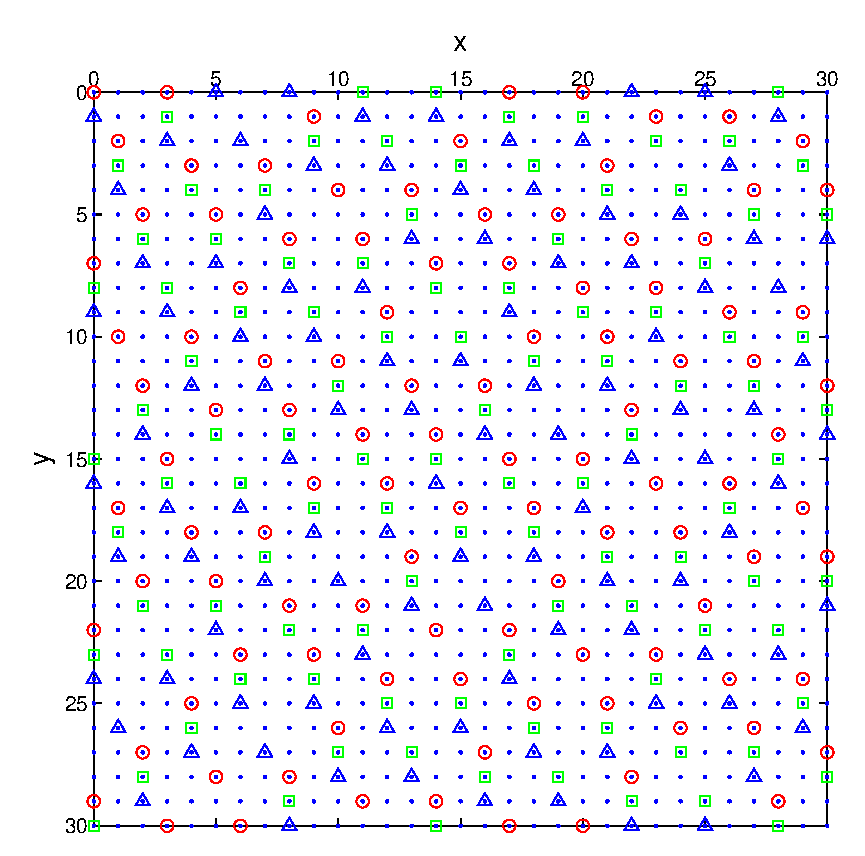
\includegraphics[width=7cm]{figure_sampling_view1.eps}
    \medskip
    \centerline{(a)}
  \end{minipage}\hfill
  \begin{minipage}[t]{0.49\linewidth}\centering
    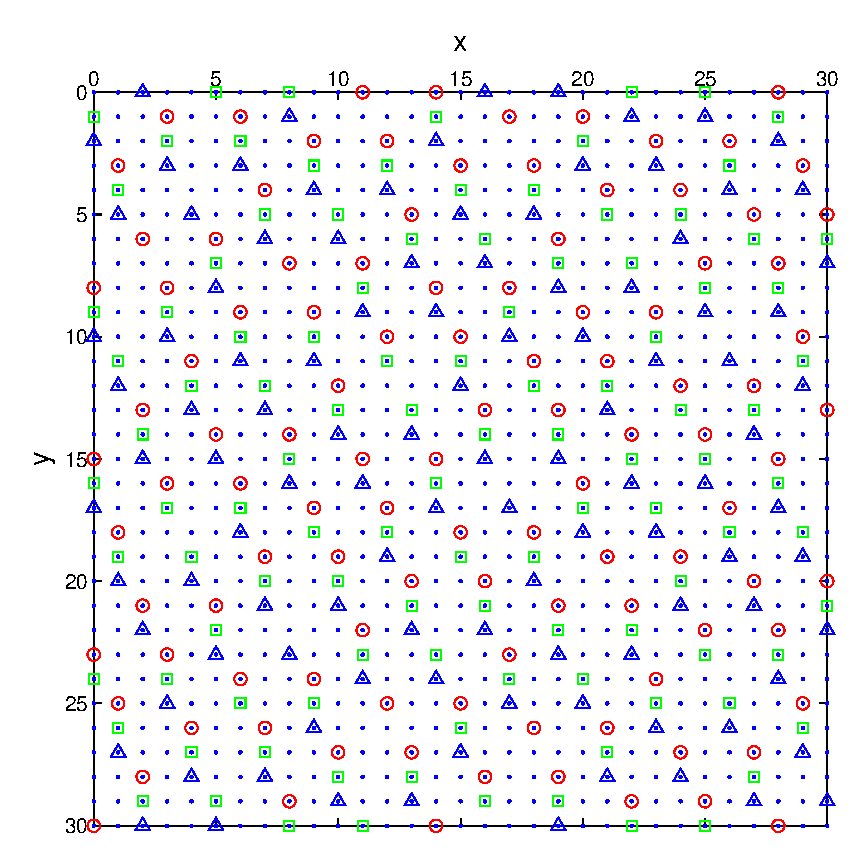
\includegraphics[width=7cm]{figure_sampling_view2.eps}
    \medskip
    \centerline{(b)}
  \end{minipage}
  \caption{Assignment of single-view intensities to RGB components: (a) view
    \#1; and (b) view \#2. }
  \label{fig:Sampling}
\end{figure}

You will also be using a lot of citations. Here is the format required in the dissertation: \cite{lamport1985:latex},\cite{Debr01}.

In all likelihood, you will need to insert tables. See one example on the next page.
\clearpage

\begin{table}[h]
	\caption{Absolute disparity error per pixel for the test data from
		Fig.~\ref{fig:Sampling} and different parameter values. In each experiment one
		parameter is adjusted while other parameters are unchanged.} 
	\centering
	\begin{minipage}[b]{0.30\linewidth}
		\centerline{$\eta=6000$, $\mu=2000$}\smallskip
		\centering
		\begin{tabular}{ccc}
			\hline
			$K$ & $u_1$ & $u_2$\\
			\hline
			3   & 0.52 &0.46\\
			7   & 0.47 &0.43\\
			10  & 0.35 &0.36\\
			12  & 0.37 &0.36\\
			\hline
		\end{tabular}
	\end{minipage}
	%
	\begin{minipage}[b]{0.34\linewidth}
		\centerline{$K=10$, $\mu=2000$}\smallskip
		\centering
		\begin{tabular}{ccc}
			\hline
			$\eta$ & $u_1$ & $u_2$\\
			\hline
			1000&0.54& 0.45\\
			3000&0.43& 0.40\\
			6000&0.35& 0.36\\
			9000&0.37& 0.37\\
			\hline
		\end{tabular}
	\end{minipage}
	%
	\begin{minipage}[b]{0.32\linewidth}
		\centerline{$K=10$, $\eta=6000$}\smallskip
		\centering
		\begin{tabular}{ccc}
			\hline
			$\mu$ & $u_1$ & $u_2$\\
			\hline
			100 &1.00&1.16\\
			1000&0.53&0.47\\
			2000&0.35&0.36\\
			3000&0.44&0.43\\
			\hline
		\end{tabular}
	\end{minipage}
	%
	\label{tab:Parameters}
\end{table}

Of course, there must be a Table of Contents at the beginning of the thesis.
\cleardoublepage

% -------------------------------------
% CHAPTER 3: CONCLUSION
% -------------------------------------
\chapter{Conclusions}
\label{chapter:Conclusions}
\thispagestyle{myheadings}

% set this to the location of the figures for this chapter. it may
% also want to be ../Figures/2_Body/ or something. make sure that
% it has a trailing directory separator (i.e., '/')!
\graphicspath{{3_Conclusion/Figures/}}

\section{Summary of the thesis}

Time to get philosophical and wordy.

IMPORTANT: In the references at the end of thesis, all journal names must be
spelled out in full, except for standard abbreviations like IEEE, ACM, SPIE,
INFOCOM, ...
\cleardoublepage

%\appendix
\begin{appendices}
\chapter{Proof of xyz}
\label{appendix}
\thispagestyle{myheadings}

This is the appendix.
\end{appendices}
%==========================================================================%
% Bibliography
\newpage
\singlespace
\bibliographystyle{apalike}

% each subdirectory can have its own BiBTeX file
\bibliography{thesis}
\cleardoublepage

%==========================================================================%
% Curriculum Vitae
\addcontentsline{toc}{chapter}{Curriculum Vitae}

\thispagestyle{empty}

\begin{center}
{\LARGE {\bf CURRICULUM VITAE}}\\
\vspace{0.5in}
{\large {\bf Joe Graduate}}
\end{center}

Basically, this needs to be worked out by each individual, however the same format, margins, typeface, and type size must be used as in the rest of the dissertation. 
 

%==========================================================================%
\end{document}
